\documentclass[../main.tex]{subfiles}
\graphicspath{{\subfix{../images/}}}
\begin{document}

  \textcolor{red}{\textbf{TO-DO}
  \begin{itemize}
    \item Breve introdução ao que será dito no referencial teórico
  \end{itemize}
  }

  \subsection{O robô quadrúpede}
  \textcolor{red}{\textbf{TO-DO}
  \begin{itemize}
    \item Breve introdução ao tópico
  \end{itemize}
  }

  \subsubsection{Apresentação e conceito geral}
  O robô quadrúpede é um sistema robótico móvel que se locomove com a ajuda de pernas. Robôs móveis podem ser divididos em três grupos, relacionados aos seus sistemas de locomoção: robôs com rodas, com esteiras e com pernas. Quando comparado aos dois primeiros, o último grupo apresenta diversas particularidades que os confere muitas vantagens quanto a mobilidade, robustez a diferentes terrenos e superação de obstáculos \cite{Biswal2021}. Robôs com rodas e esteiras apresentam boa performance em terrenos planos e conseguem navegar de forma autônoma pelo espaço, desde que haja um caminho contínuo entre os pontos de origem e destino. Robôs com pernas, por outro lado, são capazes de escolher os melhores pontos de suporte no terreno para apoiar seus pés, o que permite uma navegação em caminhos discretos (com obstáculos de grande inclinação e variação de altura) \cite{Yao2021}. Essa capacidade de se adaptar de terrenos desnivelados amplia bastante a lista de aplicações às quais esse tipo de sistema pode ser designado: industriais, militares, missões de inspeção, resgate, entre várias outras. Por outro lado, essas vantagens vêm as custa de uma maior complexidade de controle e menor estabilidade. Isso influencia no custo final do sistema, o que pode ser um impeditivo para sua aplicabilidade prática. 

  Robôs com pernas também apresentam diversas diferenças entre si, majoritariamente ligadas à quantidade de pernas que possuem. Entre eles, destacam-se os bípedes, os quadrúpedes e os hexápodes (que podem ser considerados robôs com múltiplas pernas, abrangendo todos com mais de quatro pernas). A quantidade de pernas de um robô está diretamente relacionada a sua estabilidade, capacidade de locomoção e eficiência. Os bípedes possuem baixa estabilidade, visto que se apoiam em apenas uma perna para poder andar e, portanto, necessitam de sistemas de controle complexos para poder de mover. Em contrapartida, os com múltiplas pernas possuem maior estabilidade, afinal conseguem manter pelo menos três (muitas vezes até quatro) pontos de apoio enquanto realizam um passo. Contudo, cada perna apresenta um adicional de juntas e atuadores no sistema, diminuindo a eficiência do sistema como um todo. Os quadrúpedes conseguem unir vantagens dos dois anteriores, ao apresentar um balanço entre estabilidade e eficiência. Eles possuem uma estabilidade passiva, quando estáticos, pois se apoiam em quatro pontos. Além disso, também são capazes de navegar de forma estável em baixas velocidade, movendo uma perna por vez, enquanto as outras três permanecem no solo, o que elimina a redundância e complexidade dos robôs com múltiplas pernas e aumenta sua eficiência \cite{Yao2021}.

  \subsubsection{Estrutura e design}
  Por conta das vantagens que apresentam, os robôs quadrúpedes se tornaram um grande foco de pesquisa nos últimos anos. Muitos tipos diferente de designs já foram testados, variando o tipo de perna, modelo de estrutura e número de graus de liberdade (degree of freedom (DOF)) por perna. Alguns designs de quadrúpedes com diferentes tipos de perna e modelos de estrutura podem ser vistos na figura \ref{fig:structure_design}.

  \begin{figure}[h]
    \centering
    \caption{Titulo da Figura}
    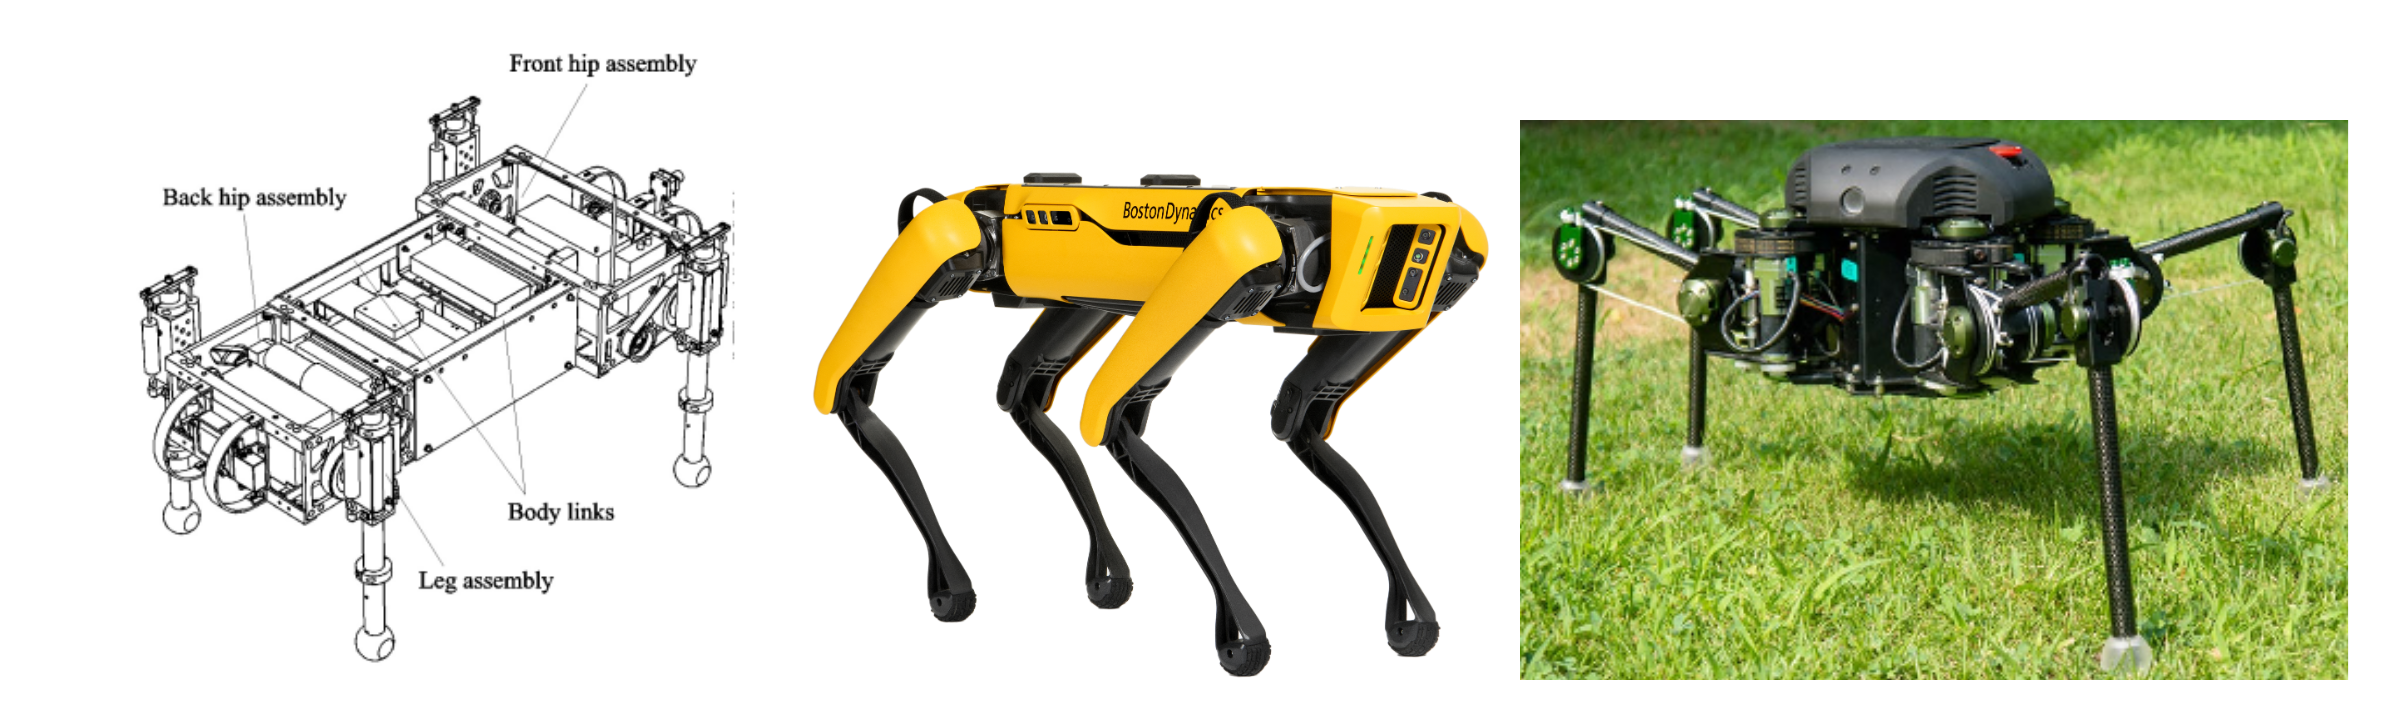
\includegraphics[width=0.48\textwidth]{structure_design.png}
    
    Fonte: XXX
    SCOUT-II / SPOT / TITAN-XIII
    \label{fig:structure_design}
  \end{figure}

  O SCOUT-II, assim como outros robôs que foram alvo de pesquisa na década de 80 por Raibert \cite{Raibert1986}, utilizam pernas prismáticas, ou lineares. Isto é, a perna possui apenas uma junta rotativa que a conecta ao corpo e uma junta prismática responsável por aumentar ou diminuir seu comprimento \cite{Zhong2019}. Essa junta prismática pode ser ativa ou passiva. Juntas ativas podem utilizar pistões ou mecanismos parafusados. Já os de junta passiva, como o SCOUT-II, possuem uma mola com amortecedor, possibilitando a locomoção do robô com base em um movimento oscilatório \cite{Talebi2007}.

  O modelo de estrutura do TITAN-XIII é chamado de sprawling type, que pode ser traduzido para tipo amplo, devido a grande amplitude de abertura das pernas. Já o modelo do Spot, da Boston Dynamics, pode ser chamado de mammal type ou tipo mamífero, por ser inspirado da postura de mamíferos quadrúpedes como cachorros e cavalos. Ambos possuem pernas articuladas com juntas rotativas, podendo variar a quantidade de juntas por perna, a depender do robô. Kitano et al., em \cite{Kitano2016}, cita algumas vantagens de cada um desses dois modelos de estrutura. O modelo mamífero é capaz de alcançar maiores velocidades, por possuir duas juntas no plano sagital. Além disso, ele também é mais eficiente, pois seus atuadores utilizam menos torque para sustentar o robô, devido à sua estrutura mais compacta, que diminui o braço de alavança sobre o qual a força peso do robô atua. Isso também lhes permite navegar em ambientes estreitos, onde um robô do tipo sprawling teria dificuldades de acessar. Este último, por sua vez, possui uma estrutura que o permite abaixar seu centro de gravidade, dando-lhe mais estabilidade de movimentação e causando menos danos ao robô em caso de quedas, o que é uma vantagem de segurança e confiabilidade. Sua estrutura larga também o permite alcançar pontos de apoio no solo mais distantes do corpo, aumentando seu polígono de suporte. Esse é o polígono paralelo ao solo, cujos vértices são os pés de apoio do robô e sobre o qual o centro de gravidade do sistema deve estar, a fim de garantir estabilidade de movimento. Uma outra vantagem de mobilidade desse tipo de quadrúpede é poder utilizar seu corpo como uma quinta perna, em algumas ocasiões.

  O modelo de estrutura de robô abordado neste trabalho será do tipo mamífero. Entre os robôs quadrúpedes que utilizam esse modelo, eles também se diferenciam quanto ao número de DOF por perna, tipos de atuadores nas juntas e configuração das pernas. Quanto à configuração das pernas, existem quatro tipos, ilustrados na figura abaixo.

  \begin{figure}[h]
    \centering
    \caption{Titulo da Figura}
    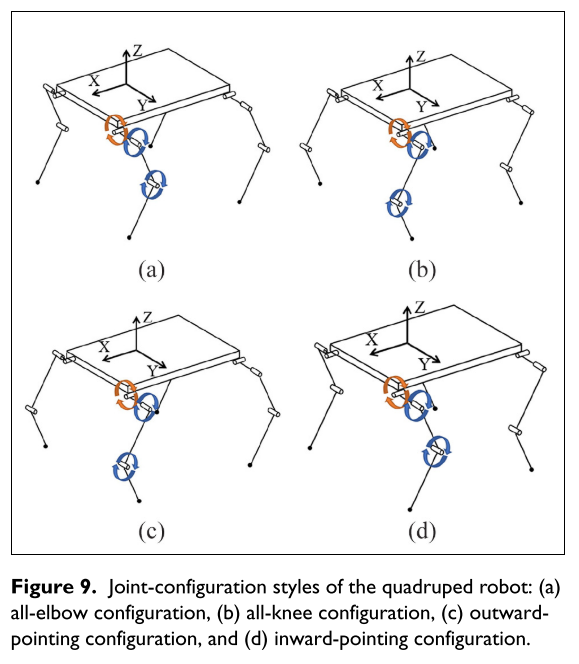
\includegraphics[width=0.48\textwidth]{joint_configurations.png}
    
    Fonte: XXX
    \label{fig:joint_configurations}
  \end{figure}

  Entre eles destacam-se o \textit{full-elbow} e o \textit{elbow-knee}. Robôs como o Spot, MIT Cheetah e Stanford Pupper utilizam a configuração \textit{full-elbow}, enquando outros como o ANYmal, StarlETH e BigDog adotam a configuração  \textit{elbow-knee}. \textbf{\textcolor{red}{\textit{Yao et al.}}} acreditam que a configuração \textit{elbow-knee} possibilita maior estabilidade, mas as características de movimento da configuração \textit{full-elbow} podem ser superiores.

  O número de juntas nas pernas, que coincide com a quantidade de DOF do robô também é um dos aspectos estudados sobre os quadrúpedes. A maioria apresenta 3 DOF por perna, o que é suficiente para que o robô consiga mover seus pés em três dimensões e realize diversos tipos de marchas. A fim de simplificar a estrutura e consequentemente o controle, alguns robôs utilizam apenas 2 DOF por perna, eliminando a junta no corpo que movimenta a perna no plano frontal. Outros buscam performances mais semelhantes ao andar de animais reais, o que aumenta a flexibilidade de movimento, justificando acrescentar uma quarta junta na perna. No entando, como já mencionado, isso aumenta a complexidade do controle e acrescenta mais atuadores ao robô, o que prejudica a eficiência.

  Essa perda de eficiência se dá porque mais atuadores significa mais consumo de energia e também mais massa. A massa do robô quadrúpede deve ser a menor possível. Quanto mais leve for o sistema, menos torque será demandado dos motores e maior sua eficiência. Além disso, a distribuição de massa do robô também deve ser considerada. A massa deve ser localizada majoritariamento no corpo, enquanto as pernas devem possuir baixa inércia. Isso as permite se mover rapidamente, sem alterar de forma significativa o centro de gravidade do robô, o que melhora a estabilidade e requer menos complexidade de controle. Possuir baixa inercia significa possuir baixa massa, porém as pernas devem ser resistentes o suficiente para suportar o peso do robô além de vários distúrbios causados pelo impacto dos pés com o chão durante a movimentação, o que pode demandar um aumento de massa. Um balanço entre massa e resistência deve ser buscado, o que reforça a necessidade de se diminuir a massa total do sistema \cite{Zhong2019}.

  \subsubsection{Atuadores}
  Robôs quadrúpedes também podem ser categorizados com base no tipo de atuadores que utilizam em suas juntas. O tipo de atuador exerce uma enorme influência na performance de movimento do robô, massa total e capacidade de \textit{payload}, assim como no sistema de controle que será utilizado das juntas. Em um estudo sobre atuadores de robôs quadrúpedes \cite{Yao2021}, \textbf{\textcolor{red}{\textit{Yao et al.}}} abordam diferentes tipos de atuadores e analisam a performance de robôs quadrúpedes que os utilizam. Os três tipos principais são: hidráulicos, atuadores elásticos em série (\textit{series elastic actuators, SEA}) e motores elétricos com redução. Robôs com atuadores hidráulicos normalmente possuem mais massa e, consequentemente, maior \textit{payload} (kg), embora sua capacidade de \textit{payload} (\%) seja mais baixa. Esse tipo de atuador possui alta potência e uma performance rápida e estável. Em contrapartida, robôs com atuadores eletromagnéticos apresentam melhor movimentação e mais agilidade, sendo capazes de realizar mais tipos de marchas. Os SEAs são formados por motores elétricos e elementos elaśticos como molas, a fim de eliminar picos de torque, permitir o melhor controle do torque nas juntas e ainda aumentar seu compliance. Entre os robôs analisados, os com SEAs apresentaram maior capacidade de \textit{payload}. Os atuadores com redução são altamente utilizados com a função de aumentar o torque nas juntas, a custo de uma perda de velocidade. Eles também possui uma performance de controle de torque satisfatória. Na comparação realizada, os robôs com esse tipo de atuador apresentaram capacidade de \textit{payload} equiparada a daqueles com atuadores hidráulicos e, em geral, menor velocidade, com exceção do Cheetah 2, que está muito acima da média nesse quesito, sendo, hoje em dia, um dos quadrúpedes mais rápidos do mundo.

  Um outro tipo de atuador utilizado em robôs quadrúpedes são os servomotores: motores DC equipados com uma caixa de redução e \textit{encoder}. Esses motores são menos adaptáveis a diferentes condições do terreno, pois fornecem baixo compliance nas juntas, e possuem baixa valocidade, limitando a agilidade do robô. No entanto, produzem alto torque e permitem um preciso controle de posição. Também são mecanismo simples, leves e de baixo custo, o que os torna adequados para projetos de pesquisa e voltados para educação. O protótipo desenvolvido nesse trabalho utiliza servomotores, pois este era o recurso disponível mais facilmente.

  \subsubsection{Processamento}
  O subsistema de processamento é o responsável por processar os dados demandados por todas as funcionalidades implementadas no robô, desde as mais fundamentais como controle das juntas e de locomoção até tarefas de mais alto-nível, como inspeção ou navegação autônoma.

  Dentre os robôs que tinham seus dados de hardware reportados no review realizado por Biswal \textbf{\textcolor{red}{[Fonte: Development of quadruped walking robots: A review]}}, a maioria utiliza sistemas operacionais (SO) baseados em RT-Linux (\textit{real-time linux}) ou outros tipos de SOs de tempo real. Sistemas em tempo real são importantes, especialmente, para robôs que embarcam os controladores das juntas nos computadores de bordo, pois eles conseguem garantir o tempo execução de todo o processamento necessário para o loop de controle, o que melhora a performance e pode ser crucial para a segurança do robô e de seus operadores. Outra solução é embarcar o controle de baixo-nível em um sistema microncontrolado que se comunica com um PC para tarefas de nível mais alto, como é feito no TITAN-XIII \cite{Kitano2016}.

  Tratando-se do processamento necessário pera realizar o controle de locomoção de robôs quadrúpedes, o controle das juntas, normalmente, é o que possui a frequência de operação mais alta, pois sua estabilidade é crítica para a operação do robô. O controle das juntas do ANYmal opera a 400 Hz \textbf{\textcolor{red}{[ANYmal - A Highly Mobile and Dynamic Quadrupedal Robot]}}, o do HyQ e o do TITAN-XIII a 1 kHz \textbf{\textcolor{red}{[Fontes: Design of HyQ -A hydraulically and electrically actuated quadruped robot, TITAN-XIII: sprawling-type quadruped robot with ability of fast and energy-efficient walking]}} e o do LittleDog a 500 Hz \textbf{\textcolor{red}{[Fontes: A Controller for the LittleDog Quadruped Walking on Rough Terrain]}}. Tarefas de mais alto nível são realizadas em frequências menores, pois possuem menor criticidade e maior custo computacional. Alguns robôs como o TITAN-XIII, o HyQ e o LittleDog executam essas tarefas em um computador externo, com uma conexão sem fio com o computador de bordo. Isso diminui a complexidade do sistema embarcado no robô e também sua massa total, porém aumenta o risco de erros de comunicação assim como a latência. O frequência de execução dessas tarefas também varia bastante para cada robô, afinal dependem do método de controle implementado em cada um. O LittleDog executa seu loop de mais alto-nível a 100 Hz \textbf{\textcolor{red}{[Fontes: AA Controller for the LittleDog Quadruped Walking on Rough Terrain]}}, o TITAN-XIII a 50 Hz \cite{Kitano2016} e o HyQ a 200 Hz \textbf{\textcolor{red}{[Fontes: Design of HyQ -A hydraulically and electrically actuated quadruped robot]}}.



  \subsection{Movimentação por marchas}
  Robôs quadrupedes se movimentam conforme uma sequência de movimentos coordenados de suas pernas que compõe uma marcha (\textit{gait}, em inglês). Em uma descrição mais detalhada, \textbf{\textcolor{red}{Song and Waldron (1989)}} afirma que: 

  \textcolor{red}{“Uma marcha é definida pelo tempo e local de colocação e levantamento de cada pé, coordenado com o movimento do corpo em seus seis graus de liberdade, para mover o corpo de um lugar para outro”.}

  Planejar a marcha de forma robusta é um aspecto fundamental para garantir que um robô com pernas caminhe por terrenos variados de forma eficiente e estável \cite{X.129}. Esta sequência de passos pode ser classificada nas seguintes categorias: periódica e aperiódica, simétrica e assimétrica. Uma marcha é chamada de periódica quando o robô segue uma sequência fixa de movimentos, de acordo com um padrão pré-planejado e considerando que todos os posicionamentos dos pés são válidos. Enquanto que durante uma marcha aperiódica, a sequência dos passos, o posicionamento dos pés e os movimentos do corpo são planejados de forma não fixa e flexível, em função da trajetória e das características do solo \textbf{\textcolor{red}{Fonte: chapter :Generation of Non-periodic Gaits, Quadrupedal Locomotion}}. De forma geral, marchas periódicas são limitadas a trajetórias pré-definidas e são ineficientes em terrenos muito irregulares \cite{X.129}. Quanto à simetria, marchas são classificadas como simétricas quando os passos dos pés dianteiros e dos pés traseiros são espaçados uniformemente no tempo. Quando algum dos pares se movimentam de forma desigual, a marcha é chamada de assimétrica \textbf{\textcolor{red}{[Fonte: M HildebrandAnalysis of the symmetrical gaits of tetrapodsFol. Biotheor., 6 (1966), pp. 9-22]}}.

  No campo da locomoção com pernas, as marchas são divididas em duas fases, stance e swing - apoio e balanço respectivamente. Durante a fase stance, ou  support, as pernas se tensionam, fixando-se no solo e impulsionam o robô para frente, movendo também o centro de massa do sistema, e o peso do robô é dividido entre as pernas de apoio. Enquanto que no swing, ou flight, as pernas de balanço se movem até os novos pontos da trajetória. Além disso, outros parâmetros são utilizados para caracterizar as marchas. O período da marcha é o tempo necessário para realizar um ciclo de movimento, ou seja, para que o robô saia da fase de suporte, movimente suas pernas e retorne à fase de suporte. O \textit{duty factor}, $\beta_i$, é a fração do ciclo do movimento em que uma perna se mantém no solo. A diferença de fase entre as pernas do robô, $\Phi_i$, é a diferença temporal normalizada entre o movimento realizado por uma perna i em relação a perna de referência. Por exemplo, uma marcha que move uma perna por vez possui diferença de fase de um quarto de ciclo. \textit{Leg stroke}, $R$, é o parâmetro que expressa a distância do pé em relação ao corpo do robô durante a fase de suporte, conforme demonstra a Figura \ref{fig:passada}. Enquanto que o \textit{stroke pitch}, é a distância entre os pés adjacentes, $P_x$ é a distância entre os centros do curso das pernas colaterais e $P_y$ é a distância entre os centros do curso das pernas contralaterais. Por fim, tem-se que o comprimento da passada, $\lambda$, de uma marcha é a distância percorrida pelo centro de gravidade do corpo ao longo de um ciclo de locomoção. Sendo que, se a marcha for periódica essa distância é definida pela relação \ref{eq:passada}.

  \begin{equation}
    \lambda=\frac{R}{\beta}
    \label{eq:passada}
  \end{equation}

  Estas variáveis são definidas para cada aplicação, de forma a atender o objetivo especifico da marcha, seja possuir maior ou menor velocidade ou ser mais ou menos estável.

  \begin{figure}[h]
    \centering
    \caption{Definições geométricas de uma marcha}
    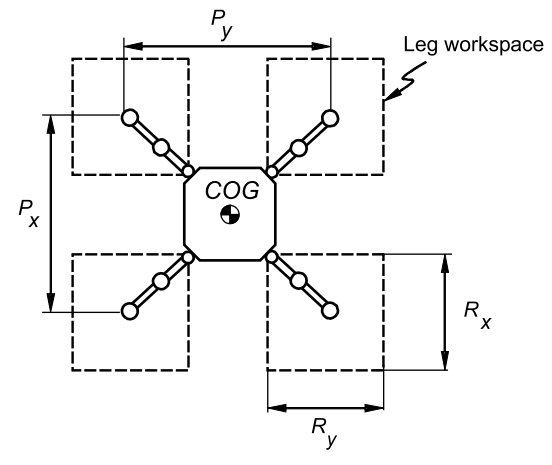
\includegraphics[width=0.48\textwidth]{passada.png}
    
    Fonte: \textcolor{red}{quadrupedal locomotion}
    \label{fig:passada}
  \end{figure}

  As marchas desenvolvidas para robôs quadrupedes são originalmente inspiradas na movimentação de animais. \textit{Walk}, \textit{trot}, \textit{pace}, \textit{gallop} são exemplos de marchas comumente utilizadas, as quais se diferenciam de forma geral pela ordem das passadas e pela duração das fases de apoio e balanço \cite{Yan2021}. Dentre estas marchas, o trote é a mais utilizada dado sua simplicidade e eficiência em uma ampla faixa de velocidade de corrida. Neste movimento as pernas diagonais se movem em conjunto enquanto as outras duas sustentam o corpo e se movem para trás \cite{X.118}. Durante o trote é observado também uma boa estabilidade, pois a linha de apoio entre os pés passa diagonalmente por debaixo do corpo \textbf{\textcolor{red}{Fonte: The Mechanics of and Robotic Design for Quadrupedal Galloping}}. O galope, diferente das demais, é uma marcha assimétrica e é a que confere maior velocidade aos animais, utilizada por exemplo por guepardos e cavalos. É caracterizada por mover os pares dianteiros sequencialmente e em seguida os traseiros, porém, o movimento possui uma diferença de fase entre as duas patas dianteiras maior do que as patas traseiras, de forma que dois pés não tocam o chão ao mesmo tempo \textbf{\textcolor{red}{Fonte: M. Hildebrand. The adaptive significance of tetrapod gait selection. American Zoologist, 20:97–103, 1977.}}. A marcha pace consiste em mover o par de pernas do mesmo lado em fase e é geralmente observada em animais quadrupedes de pernas longas, como girafas e camelos, pois impede que as pernas colidam durante o movimento \textbf{\textcolor{red}{Fonte: Pace Running of a Quadruped Robot Driven by Pneumatic Muscle Actuators: An Experimental Study}}. Assim como o trote, a diferença de fase é metade de um ciclo, porém é menos estável, uma vez que desloca a linha de apoio para as extremidades do robô. Já durante a marcha walk, ou crawl, três pernas se mantêm em contato com o solo e uma se movimenta, assim como fazem as tartarugas, de modo que a diferença de fase entre as pernas é um quarto de ciclo \cite{X.110}. Esta movimentação confere maior estabilidade, porém reduz a velocidade da caminhada. \textcolor{red}{Citar o polígono de suporte aqui, para explicar a estabilidade, dar um destaque maior já que iremos utilizar.}


  \subsection{Controle de locomoção}
  \textcolor{red}{\textbf{TO-DO}
  \begin{itemize}
    \item Breve introdução ao tópico
  \end{itemize}
  }

  \subsubsection{Modelo cinemático}
  Um modelo cinemático descreve a relação entre as variáveis de juntas e a posição e orientação do end-efector. Durante a análise cinemática de um robô quadrupede, é afirmado que o sistema consiste em um corpo rígido composto por quatro pernas com três graus de liberdade \textbf{\textcolor{red}{[Fonte: p]}}. A fim de mover este corpo por uma dada trajetória, é necessário um movimento coordenados das juntas \textbf{\textcolor{red}{[q]}}. Logo, o modelo cinemático descreve a relação entre as variáveis de juntas, a posição do pé e suas derivadas. Considerando que as juntas são rotacionais, a variável de junta é definida como o ângulo entre os elos ligados por tal junta.

  O modelo cinemático de um corpo articulado em malha aberta pode ser dividido em dois problemas: cinemática direta e cinemática inversa. Durante a análise de cinemática direta, as variáveis das juntas fornecem a posição do \textit{end-efector}, enquanto que a cinemática inversa é o processo de encontrar os valores das juntas de acordo com a posição e orientação do end-efector. Para mover o pé do robô quadrúpede até uma posição desejada, é necessário determinar os valores rotacionais das juntas das pernas com análise de cinemática inversa.

  O corpo inteiro do robô é levado em consideração na modelagem, as coordenadas do seu centro de massa, assim como os parâmetros de comprimento e da largura do robô e os comprimentos dos elos, são utilizados para descrever a posição de cada perna. Percebe-se que as pernas estão em orientações diferentes mas possuem a mesma estrutura, logo é suficiente analisar a cinemática inversa de uma perna [x]. Neste processo, é frequentemente utilizado os parâmetros de Denavit-Hartenberg como uma forma sistemática  de escrever a cinemática direta, a fim de obter as matrizes de transformação requeridas para a realizar cinemática inversa.

  A análise cinemática inversa é frequentemente realizada por meio de métodos analítico, como em \textbf{\textcolor{red}{[Fonte: p]}}, mas pode ser empregado uma abordagem geométrica. As equações que expressam a posição angular das juntas são, entretanto, não lineares e não são todas as expressões que possuem uma solução física possível.  Além disso, pode haver mais de um conjunto de posições dos pés que fornecem a mesma posição final \textbf{\textcolor{red}{[Fonte: p]}}.

  Além disso, pode haver mais de uma configuração de ângulos de juntas que fornece a mesma posição final \textbf{\textcolor{red}{[Fonte: p]}}.

  \textbf{Denavit-Hartenberg}
  
  \textcolor{red}{\textbf{TO-DO}
  \begin{itemize}
    \item Para a versão final, acho que cabe a gente colocar uma imagem aqui com um exemplo dos frames e indicando o que são essas 4 variáveis. Pode ser um exemplo com 2 DOF só, apenas para facilitar o entendimento.
  \end{itemize}
  }

  \textcolor{red}{Jacques Denavit e Richard Hartenberg} introduziram em 1995 [l] uma convenção para descrever sistematicamente a posição e a orientação relativa de um conjunto de elos e juntas consecutivos. Trata-se de uma análise difundida na robótica de manipuladores e é empregada de forma análoga em estudos de cinemática de robôs com pernas, considerando que as pernas funcionam como um manipulador, de forma que o pé representa o end-efector.

  No processo, as juntas são consideradas como frames no espaço 3D e, observando a geometria da perna do robô, é possível alcançar relações de translações e rotações entre estes frames, que são independentes do movimento da perna. Dessa forma, concatenar as equações entre os frames consecutivos resulta em uma matriz homogênea que transforma as coordenadas do pé, junta n, até a junta de quadril, junta 0. 

  Durante o procedimento de D-H, inicialmente, é definido um sistema de coordenadas, então todas as juntas são localizadas para determinar a direção do eixo z, que deve condizer com o eixo de rotação da junta. Em seguida são definidas as posições do frames e posicionados os eixos x e y, por meio a regra da mão direita. Com esta convenção são utilizadas apenas quatro variáveis: $a_i$, distância em módulo entre os eixos, ao longo do eixo x; $\alpha_i$, ângulo entre os eixos, medido em torno do eixo x; $d_i$, distância entre os eixos ao longo do eixo z; e $\theta_i$, ângulo entre os eixos em torno do eixo z.

  O resultado consiste em um poderoso e confiável procedimento analítico pois são baseados em matrizes algébricas consistentes.

  \subsubsection{Etapas do controle e conceitos gerais}
  A locomoção de robôs quadrúpede, em geral, segue uma sequêcia de passos. Essa sequência depende fortemente do design do robô e do tipo de marcha que será utilizada. Raibert, em uma das publicações mais marcantes para a pesquisa de robôs com pernas \cite{Raibert1986}, propõe um método de controle baseado em três etapas: controle de salto, controle de velocidade e controle de postura do corpo. Essa pesquisa foi desenvolvida com robôs de pernas rígidas, semelhantes ao SCOUT-II, que utilizam uma junta prismática nas pernas e uma rotativa junto ao corpo. Esse sistema de controle baseava-se na implementação independente de três controladores que, agindo em conjundo, controlariam a locomoçãodo robô de forma estável, a partir da velociade, a altura de salto do robô e o ângulo do corpo. Essa estratégia de controle foi utilizada para controlar robôs com uma, duas e quatro pernas, tanto no espaço 2D quanto 3D. Sua premissa básica era a de que apenas uma perna estaria em \textit{stance} ou em \textit{swing} por vez. A fim da satisfazer essa premissa para robôs com mais duas pernas, foi proposto o conceito de pernas virtuais. Isto é, um conjunto de pernas deve realizar igual comportamento quando em \textit{swing} e \textit{stance} e as fases de swing e stance de cada conjunto devem ser alternadas. Dessa forma, é possível modelar o robô como possuindo apenas duas pernas virtuais, cada uma representando um dos dois conjuntos de pernas físicas em igual movimento. Tratando-se do quadrúpede, essa premissa pode ser satisfeita considerando duas pernas como uma perna virtual. O ponto de conexão dessa perna virtual no corpo do robô é localizado no centro da reta unindo ambos os pontos de conexão com o corpo das pernas físicas. Utilizando esse conceito, pode-se utilizar marchas simétricas como o \textit{trot}, \textit{pace} e \textit{bound}.

  A estratégia de controle em três etapas proposta por \textcolor{red}{Raibert} foi responsável por locomover robôs com pernas rígidas de maneira simples, porém esses robôs não tinham autonomia de energia (eram alimentados por um capo umbilical a uma fonte extera) e apenas operavam no terreno plano e controlado do laboratório. A fim de possibilitar a operação de robôs com pernas em terrenos desnivelados e de difícil mobilidade, os robôs quadrúpes passaram por modificações de design e estratégias de controle. Outro marco nessa área de pesquisa foi o robô BigDog, cujo trabalho foi publicado por \textbf{\textcolor{red}{Raibert et al.}} \textbf{\textcolor{red}{[Fonte: BigDog, the Rough-Terrain Quadruped Robot]}}. O BigDog é um robô quadrúpede com 4 DOFs por perna movido por atuadores hidráulicos. Essa maior flexibilidade de movimentação das pernas permite controlar a locomoção do robô sem que este precise saltar, sendo possível, então, dividir o controle de locomoção em duas etapas principais: controle de stance e controle de \textit{swing}. Assim, a velocidade do robô, postura do corpo e altura do corpo em relação ao chão, que é equivalente ao controle de altura do salto, seriam estados controlados por esses dois controladores, o de \textit{stance} e o de \textit{swing}.

  O controle de stance é responsável por controlar o comportamento das pernas na fase de stance, cuja responsabilidade é utilizar a tração com o terreno para manter o corpo em equilíbrio e direcioná-lo na direção desejada de locomoção. Enquanto isso, o controle de \textit{swing} é responsável por controlar as pernas em swing, de forma que os pés (\textit{end-effectors}) sigam a trajetória de um passo até o próximo ponto de apoio no chão. Para robôs quadrúpedes, ambos os controladores operam simultaneamente, mas em pernas diferentes, seguindo o princípio, muitas vezes, das pernas virtuais. A marcha utilizada pelo robô é dada por quando e quais pernas estão em cada fase: pernas diagonais em stance ou \textit{swing}, ao mesmo tempo, caracterizam a marcha \textit{trot}, por exemplo. Portando, deve-se ser capaz de coordenar o comportamento das pernas entre ambas as fases. O componente do sistema de controle com essa responsabilidade é o planejador de marchas (\textit{gait planner} ou \textit{gait scheduler}).

  Como cada perna se comporta durante cada fase é algo que varia com o método de controle utilizado por cada robô, mais ainda é possível elencar semelhanças gerais. Na fase de \textit{swing}, calcula-se o local do próximo ponto de apoio dos pés, com base na velocidade desejada para o robô, e uma trajetória de passo até esse ponto. Essa trajetória pode ser uma curva senoidal \cite{X.118}, triangular \textbf{\textcolor{red}{[Fontes: github.com/mike4192/spotMicro /stanfordroboticsclub/StanfordQuadruped]}}, de Bezier \textbf{\textcolor{red}{[Fonte: hackaday.io/project/171456-diy-hobby-servos-quadruped-robot]}}, cicloidal \cite{Shi2021} \cite{X.58}, entre outras, e o componente encarregado por calculá-la é o planejador de trajetórias. Uma consideração comum é a de que as trajetórias das pernas em cada fase são independentes, de tal forma que o estado do pé no momento em que toca o solo se torna um dos pontos chave para a estabilidade do robô  \cite{X.118}. Nesse sentido, a trajetória cicloidal ganha destaque, porém outras curvas podem ser utilizadas para gerar diferentes perfis de aceleração e velocidade dos pés durante uma passada. Curvas como a de Bezier, por exemplo, possuem grande flexibilidade, o que permite se criar várias trajetórias distintas que podem ser geradas em tempo-real, como é feito em  \textbf{\textcolor{red}{[Fonte: Dynamics and Domain Randomized Gait Modulation with Bezier Curves for Sim-to-Real Legged Locomotion]}}.

  Já na fase de \textit{stance}, as pernas devem manter o robô em equilíbrio ao mesmo tempo que direcionam o corpo na direção de locomoção desejada. Para isso, alguns trabalhos utilizam trajetórias de um formato fixo para os pés, assim como na fase de \textit{swing}, porém, não necessariamente com o mesmo formato de curva usado nesta última \cite{X.118} \cite{X.58}. Além disso, controladores de equilíbrio também podem ser implementados. Esses controladores visam estabilizar o pitch e roll do robô \cite{Shi2021} \textbf{\textcolor{red}{[Fontes:hackaday.io/project/171456-diy-hobby-servos-quadruped-robot, StanfordQuadrupedm notspot-sim-cpp ]}} ou até mais graus de liberdade, como em \cite{Chen2020140736} \cite{X.134} \cite{Zhang2016284}. Eles podem ser baseados na leitura de sensores inerciais ou no equilíbrio das forças de contato com o solo que atuam em cada perna, por exemplo.


  \subsubsection{Métodos de controle}




  \subsection{Benchmarking}

  
\end{document}
